Hauptziel der Arbeit war es alle Komponenten des AFEs gut zu vermessen und ihre Funktionalität zu verifizieren.

\subsection{Setup \& Software}
Zum Messen wurden verschiedenste Gerätschaften verwendet. Manche konnten zur Automatisierung der Messungen per Skript angesteuert werden. Alle Geräte sind im Folgenden kurz erwähnt und beschrieben, da die Ansteuerung direkt mit deren Funktionsumfang zusammenhängt.

\subsubsection*{Hauptlabornetzgerät}
Hier handelt es sich um ein gewöhnliches Labornetzgerät, welches sich leider nicht fernsteuern lässt. Es speist bei den Versuchen lediglich das AFE mit 5V und übernimmt keine weitere Funktion. Es taugt für diese Funktion gut.

\subsubsection*{LeCroy wavesurfer 3054}
Das Oszilloskop ist hier um die Signalen genauer zu beobachten. Für genaue Messungen der Verstärkung und Eingangsimpedanz der Schaltung wird zwar ein VNA verwendet, jedoch misst dieser immer nur einen RMS-Wert. Um genaue Signalverläufe zu beobachten und zum Beispiel zu ermitteln ob der Sinus vom Eingang am Ausgang überhaupt noch ein Sinus ist, wird das Oszilloskop verwendet. Es wird bei Bedarf per Hand bedient und wurde nicht per Skript angesteuert.

\subsubsection*{Arduino Due}
Da zur Ansteuerung des verwendeten DACs $I^2C$ verwendet wird, war eine Schnittstelle die $I^2C$ spricht unabdingbar. Statt bereits VHDL für das FPGA zu schreiben und eine weitere Baustelle zu eröffnen, wurde ein Arduino verwendet. Es ist relativ einfach, diesen dazu zu bringen, $I^2C$ zu sprechen. Die Spannung des DACs kann somit vor der Messung eingestellt werden. Danach kann ungestört gemessen werden, ohne dass der Bus dazwischenplappert und die Messungen verfälscht. Das ganze kann vom PC aus per UART gesteuert werden.
Leider wurde nach ersten Versuchen die Vermutung angestellt dass der DAC zusätzliches Rauschen mit sich bringt, weswegen im weiteren Verlauf der Messungen mit einem präzisen Labornetzgerät agiert wurde.

\subsubsection*{Aim-TTi PL303}
Dieses Labornetzgerät kann per PC angesteuert werden. Hier war wichtig, dass das Netzgerät Spannungen auf Milivolt genau einstellen kann.
Das Ansteuern per PC geschieht über das Netzwerk oder UART. Das Gerät wird über beide Schnittstellen mit LXI angesteuert. LXI ist ein textbasiertes Protokoll und damit menschenleserlich und einfach zu implementieren. Es wurde UART gewählt, da es per Netzwerk Probleme mit der Firewall gab. Dies ist möglich obwohl LXI eigentlich für LAN gedacht ist.

Zur Ansteuerung wurden einfache Python-Klassen geschrieben, welche die Parameter der Messgeräte lesen und setzen können. Das Python-Objekt welches per Gerät instanziert wird, hat dabei keinerlei Zustand. Jegliche Zustände werden auf dem Gerät selber verwaltet. Somit können auch jederzeit am Gerät selber Einstellungen vorgenommen werden und das Python-Interface kriegt diese ohne Schwierigkeiten mit und stellt diese angenehm über Variablen wie gewohnt zur Verfügung.

\subsubsection*{Agilent E5071B}
Der Vector Network Analyzer (VNA) wird dazu verwendet ein Signal mit bekanntem Pegel und Frequenz in ein Zweitor (Mehrtor ist auch möglich, aber in diesem Falle nicht gewünscht) zu geben und am Eingang, sowie am Ausgang zu messen, wie viel von dem Signal noch übrig ist. So kann leicht das ganze System vermessen werden.

Zum Glück konnte für die Messungen ein sehr gutes Gerät von HP verwendet werden. Es hat ein sehr einfaches Benutzerinterface und lässt sich zudem per PC ansteuern. Hier gibt es mehrere Varianten wie dies geschehen kann. Es wurde wieder UART und LXI gewählt. Somit gab es nicht viel umzustellen, um auch den VNA anzusprechen. Natürlich wurden nur Python-Schnittstellen für die Funktionen, welche auch verwendet wurden, implementiert um nicht den Zeitrahmen zu sprengen.

Das verwendete Gerät kann von 300kHz bis 8.5GHz messen und ist daher bestens geeignet. Zudem hat es eine Toleranz bis 10 VDC am Messeingang, was perfekt ist, falls man bei ersten Experimenten einmal einen Fehler macht. Leider hat der VNA als Untergenze -55dBm was er an Signal erzeugen kann. Deswegen wurde für Messungen mit der kompletten Verstärkerstufe ein -10dB Dämpfungsglied verwendet, welches das Signal noch einmal verkleinert. Für die Impedanzausmessung des AD8331 wurde auf das Dämpfungsglied verzichtet, da dies natürlich in komplett falschen Messresultaten endet.

\subsection{Erste Messungen}

Mit einer ersten bestückten Leiterplatte wurden daher mit dem Oszilloskop erste Messungen durchgeführt, welche eine generelle Funktionstüchtigkeit bezeugten. Diese war gar nicht zufriedenstellend.

\begin{figure}[H]
\begin{center}
    \includegraphics[width=1\textwidth]{data/images/messungen/erste_messung}
    \caption{Erste Messungen des Gesamtsystems. Inkorrekt terminiert. Mit dem Oszilloskop gemessen.}
    \label{fig:messungen_erste}
\end{center}
\end{figure}

Diese Kurve sieht wahnsinnig unschön aus. Gerade bei den Peaks gibt es fiese Ausreisser. Und was ebenfalls nicht zu vernachlässigen ist, sind die 180 Grad Phasenverschiebung.
Auch sieht man hier, dass der Input des Funktionsgenerators ziemlich viel Rauschen hat, welches sich auch in Grafik \ref{fig:messungen_zweite} zeigt.
Dort sieht man gut, dass der Input ziemlich rauscht. Deswegen haben wir versucht N und P voneinander zu subtrahieren. Und so das Rauschen zu eliminieren. Dies hat sogar relativ gut geklappt. Natürlich ist das nicht ganz sauber, ging aber für eine erste Verifikation sehr gut.

\begin{figure}[H]
\begin{center}
    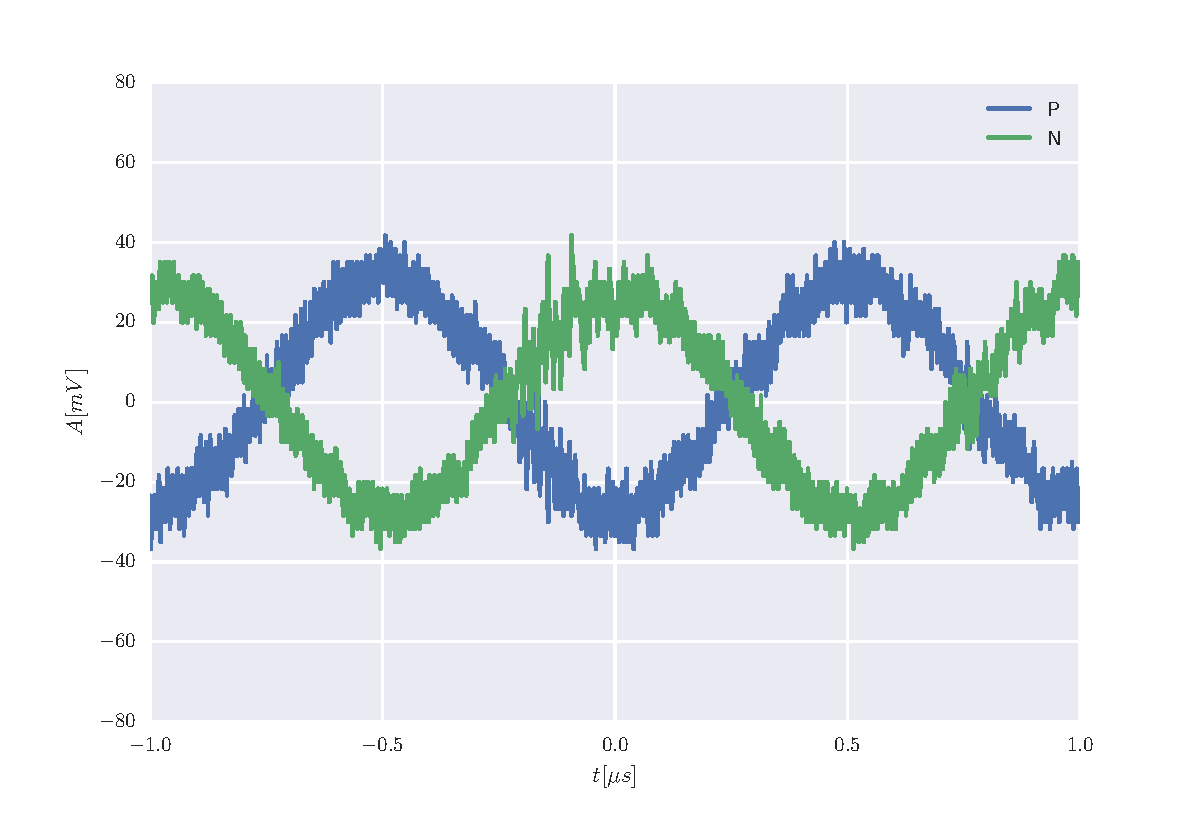
\includegraphics[width=1\textwidth]{data/images/messungen/zweite_messung_NP}
    \includegraphics[width=1\textwidth]{data/images/messungen/zweite_messung_INOUT}
    \caption{Erste Messungen des Gesamtsystems. Inkorrekt terminiert. Mit Oszilloskop gemessen.}
    \label{fig:messungen_zweite}
\end{center}
\end{figure}

Bei diesen Messungen war jedoch das DUT nicht korrekt terminiert. Dies war einer der Knackpunkte zum Anfang. Es war uns bekannt, dass Leitungen in diesem Gebiet der Elektronik korrekt terminiert werden müssen. Wenn das DUT nicht korrekt belastet wird, können ungewollte Effekte auftreten. Deswegen sind diese ersten Messungen mit Vorsicht zu geniessen und dürfen nur als Anhaltspunkt und nicht als exakte Messung angenommen werden.

Eigentlich wären zur korrekten Terminierung und Umwandlung in ein single-ended Signal, wie im Abschnitt \ref{subsec:Leiterplattendesign} beschrieben, Baluns vorgesehen. Diese sind jedoch relativ schwer zu kriegen und sind dann relativ teuer. Deswegen wurde eine günstigere Lösung gesucht. Diese wurde in der in \ref{fig:terminator} dargestellten Schaltung gefunden.

\begin{figure}[H]
\begin{center}
    \begin{circuitikz}
        \draw[dotted] (-1, 0) 
        node[rground, rotate=-90]{}
        to[V,v=$U_q$, *-] (-1,2)
        to[short] (1,2);

        \draw (1,2)
        node[ocirc]{}
        to[short] (2,2)
        to[R=$222\Omega$] (4,2)
        to[short] (6, 2)
        node[ocirc]{};

        \draw (5,2)
        to[R,l_=$65\Omega$, *-*] (5,0)
        node[rground, rotate=-90]{};

        \draw[dotted] (6, 2)
        to[short] (7, 2)
        to[R=$50\Omega$] (9,2)
        to[short] (9, 0)
        node[rground]{};

        % Lower side

        \draw[dotted] (-1, 0)
        to [V,v_=$U_q$] (-1,-2)
        to[short] (1,-2);

        \draw (1,-2)
        node[ocirc]{}
        to[short] (2,-2)
        to[R=$250\Omega$] (4,-2)
        to[short] (5, -2)
        to[short] (5, 0);

        % Boxes

        \draw[dashed] (-2, 4)
        to[short] (1, 4)
        to[short] (1, -4)
        to[short] (-2, -4);

        \draw (-1, -3) node{DUT};
        \draw[->] (-1, 3) -- (0.5, 3) node [pos=0.66,above,align=center]{$250\Omega$};

        \draw[dashed] (10, 4)
        to[short] (6, 4)
        to[short] (6, -4)
        to[short] (10, -4);

        \draw (9, -3) node{VNA};
        \draw[->] (9, 3) -- (7.5, 3) node [pos=0.66,above,align=center]{$50\Omega$};

    \end{circuitikz}
    \caption{Terminierung des AD8331 zur Messung mit single-ended Geräten die 50 $\Omega$-Terminierung haben.}
    \label{fig:terminator}
\end{center}
\end{figure}

Damit sieht der AD8331 die gewünschten 250 $\Omega$ auf beiden Ausgängen des differentiellen Signales. Zugleich sieht der VNA dabei seine gewünschten 50 $\Omega$.
Diese Lösung profitiert zwar nicht von der Störungseliminierung eines differentiellen Signales, ist jedoch für den Rahmen dieses Projektes mehr als ausreichend.

Was jetzt noch beachtet werden muss, ist der Spannungsteiler, der durch diese Schaltung am Ausgang vorgeschaltet wird.
So müssen Messresultate jeweils mit $\frac{1}{a}$ multipliziert werden wobei $a$ in Gleichung \ref{eq:a_AD8331} gegeben ist.

\begin{equation}
    a = \frac{R_L}{R_S + \sqrt{R_S(R_S - 2R_L)})} = 0.1127, R_L =50, R_S = 250
    \label{eq:a_AD8331}
\end{equation}

Dieser Wert hat noch einen kleinen Fehler, da Widerstände nur endlich genau sind. In der Fehlerrechnung \ref{eq:fehler_a_AD8331} wurde ein Fehler von ±1 für $R_S$ und $R_L$ angenommen. Dies ergibt einen Relativen Fehler von 1.86\%, was akzeptabel erscheint.

\begin{equation}
    \Delta a = \frac{R_s - R_L}{-2R_S\sqrt{R_S(R_S - 2R_L)}} = 0.0021, R_L = 50±1, R_S = 250±1
    \label{eq:fehler_a_AD8331}
\end{equation}

Mit der korrekten Korrektur des gemessenen Wertes wurde nun je eine kleine Messreihe durchgeführt. Diese ist in Grafik \ref{fig:kaputtes_AFE} zu sehen. Wie man hier unschwer erkennen kann gibt es einen signifikanten Unterschied je nach Terminierung.
Leider ist her auch unschwer zu erkennen, dass der HI/LO Pin keinerlei Einfluss auf die Verstärkung hat. Während dies bei ersten Messungen noch funktionierte, ist dies in diesem Fall nicht mehr funktional. Es scheint als wäre es ein Defekt an der Hardware.

\begin{figure}[H]
\begin{center}
    \includegraphics[width=1\textwidth]{data/images/messungen/kaputtes_AFE}
    \caption{Erste Messungen des kaputten A8331.}
    \label{fig:kaputtes_AFE}
\end{center}
\end{figure}

Die ersten Messungen sind aus diesem Grunde nicht mehr zu verwenden, ausser zur Verifikation genereller Funktionalität. Ein zweites PCB wurde aus diesem Grund bestückt und vermessen. Dieses hat keine erkennbaren Defekte und liefert anständige erste Ergebnisse wie in \ref{fig:ganzes_AFE} ersichtlich. Diese sind im Folgenden dokumentiert.

\begin{figure}[H]
\begin{center}
    \includegraphics[width=1\textwidth]{data/images/messungen/ganzes_AFE}
    \caption{Erste Verifikation des A8331.}
    \label{fig:ganzes_AFE}
\end{center}
\end{figure}

Die Inputimpedanz des A8331 sieht gut aus, wie aus Grafik \ref{fig:Z_in_A8331} unschwer geschlossen werden kann.

\begin{figure}[H]
\begin{center}
    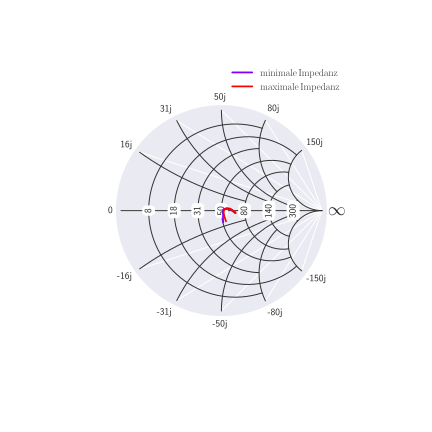
\includegraphics[width=1\textwidth]{data/images/messungen/input_Z_A8331}
    \caption{Inputimpedanz des A8331. Es sind jeweils die minimale und maximale gemessene Impedanz über alle Verstärkungen gesehen zu einer Frequenz dargestellt.}
    \label{fig:Z_in_A8331}
\end{center}
\end{figure}

Die Verstärkung sieht sehr gut aus wie Grafik \ref{fig:T_A8331} zeigt. Die Differenz zum Soll ist stets kleiner als ein Dezibel. In Anbetracht des Umstandes, dass das Datasheet lediglich variable Verstärkungen auf 0.5 dB genau garantiert, ist weniger als 1 dB Abweichung extrem gut. Zudem muss berücksichtigt werden, dass das Datasheet einen Verlust auf der externen Beschaltung von 0.4 dB zwischen den Pins LON und VOL sowie LOP und VOH spezifiziert.
Somit sieht die Kurve sogar noch viel besser aus.
Hier ist noch anzumerken, dass die Kurve um den Faktor $\frac{1}{a}$ und einen Faktor 2 korrigiert wurde. Der Faktor kommt daher, dass das differentielle Signal nur die halbe Signalamplitude hat. 

\begin{figure}[H]
\begin{center}
    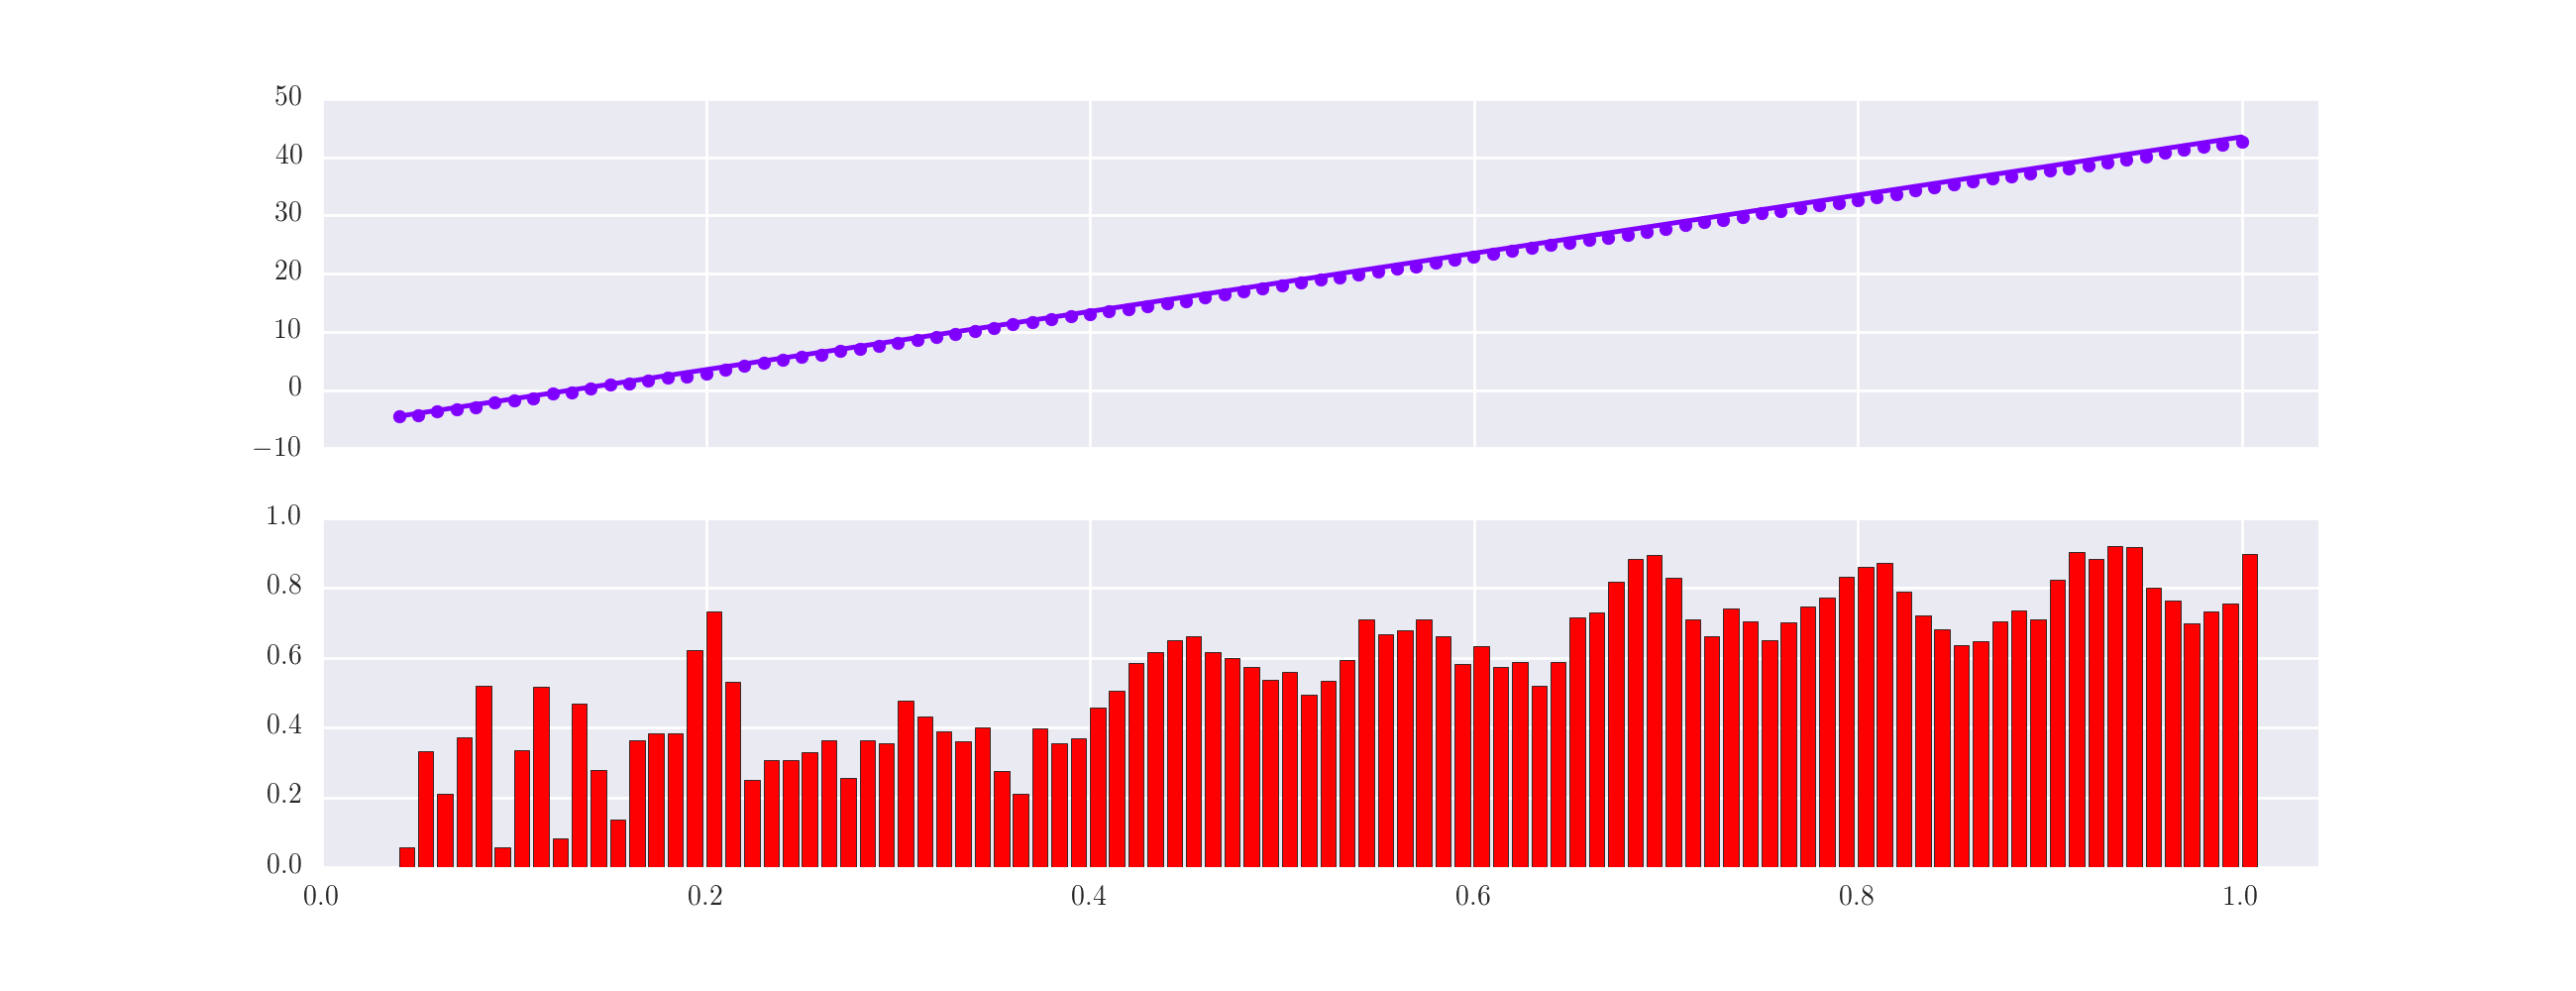
\includegraphics[width=1\textwidth]{data/images/messungen/vga_2016-12-22_30dBm_transmission2}
    \caption{Verstärkung des AD8331 gemittelt über einen 50 MHz Sweep. Ist und Soll gegenübergestellt. Zudem die Differenz zu jedem Wert.}
    \label{fig:T_A8331}
\end{center}
\end{figure}

Bei allen Messungen mit dem zweiten PCB ist der DAC nicht verbaut. Dies, da der Verdacht bestand, dass dieser eventuell Rauschen mit sich bringt, was nach der Erkenntnis, dass der AD8331 auf dem ersten Board tatsächlich kaputt ist, nicht mehr so wahrscheinlich ist. Er wurde durch eine externe Spannungsversorgung ersetzt. In weiteren Versuchen soll dieser natürlich noch genau evaluiert werden.

\subsection{ISL55210}

Da die Messungen so gut herauskamen, wurde angenommen, dass somit der AD8331 als Input für weitere Messungen am ISL55210 verwendet werden kann, um weiterhin auf einen Balun verzichten zu können. Mit einem twisted Pair wurden die beiden Stufen also verbunden. So kann die Inputimpedanz des ISL55210 zwar nicht mehr gemessen werden, hier reichte die Transmission jedoch völlig.

Im Plot \ref{fig:T_broken_ISL55210} sieht man das Verhalten des ISL55210. Sehr unschön. Es gibt aber drei interessante Dinge zu sehen.
Erstens stimmen die gemessenen Verstärkungen über den Frequenzsweep gemittelt gut mit dem Datasheet überein wie man in Grafik \ref{fig:T_broken_mean_ISL55210} sieht.

\begin{figure}[H]
\begin{center}
    \includegraphics[width=1\textwidth]{data/images/messungen/vga_lna_2016-12-22_50dBm_20dB_transmission3}
    \caption{Verstärkung des AD8331 und ISL55210 50 MHz Sweep bei 10 verschiedenen Verstärkungen.}
    \label{fig:T_broken_ISL55210}
\end{center}
\end{figure}

\begin{figure}[H]
\begin{center}
    \includegraphics[width=1\textwidth]{data/images/messungen/vga_lna_2016-12-22_50dBm_transmission2}
    \caption{Verstärkung des AD8331 und ISL55210 gemittelt über einen 50 MHz Sweep. Ist und Soll gegenübergestellt. Zudem die Differenz zu jedem Wert.}
    \label{fig:T_broken_mean_ISL55210}
\end{center}
\end{figure}

Dies kann ein Zufall sein. Was aber viel interessanter ist, dass die Kurve zwar sehr komisch ausschaut, aber überhaupt nicht wie jene, welche beim Vorgängerprojekt gemessen wurde, wie man unschwer in Grafik \ref{fig:ganzes_system_vorganger} erkennen kann.

\begin{figure}[H]
\begin{center}
    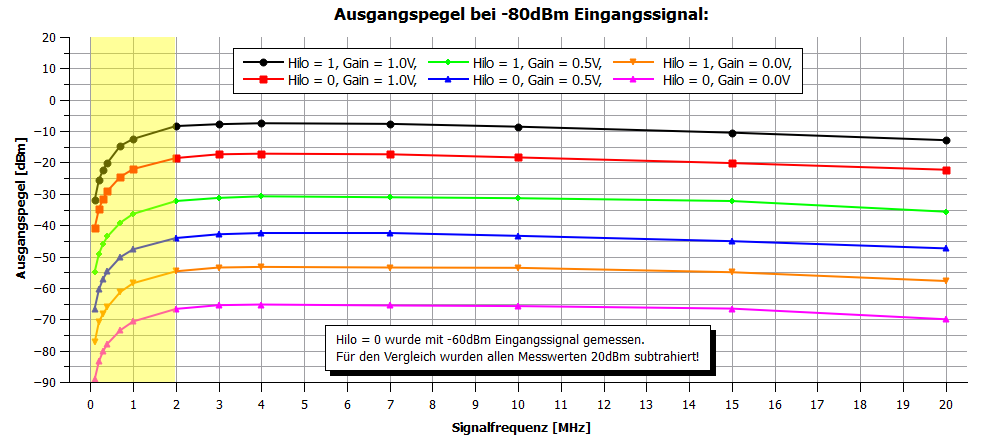
\includegraphics[width=1\textwidth]{data/images/ganzes_system_vorganger}
    \caption{Verstärkung des AD8331 und ISL55210. Gemessen im Vorgängerprojekt\cite{SDRprev}.}
    \label{fig:ganzes_system_vorganger}
\end{center}
\end{figure}

Bei dieser Kurve gibt es einen unerwarteten Abfall bei 2 MHz abwärts, wofür in der Vorgängerarbeit das aktive Impedanzmatching beschuldigt wurde. Dieses Verhalten konnte in den gemachten Messungen nicht nachvollzogen werden. Im Gegenteil, es wird ein starker Anstieg gemessen in diesem Bereich.

Ein dritter Punkt ist, dass der Verstärker einen unerwarteten Abfall hat je höher die Frequenz ist. Laut Datasheet sollte der Verstärker locker bis 100MHz um 28.5 dB verstärken. Die Kurve müsste relativ gerade ausfallen. Erst war der Gedanke da, dass es nur ein Fehler in diesem Projekt ist. Wie sich aber zeigt bestand dieses Verhalten schon im Vorgängerprojekt, wurde jedoch nicht explizit bemerkt oder wenigstens nicht erwähnt.

Erst viel zu spät wurde dann wenigstens noch bemerkt, dass der AD8331 völlig falsch belastet wurde, da nach der Einzelmessung des AD8331 die Widerstände R7 und R8 auf 0 $\Omega$ belassen wurden, statt diese korrekterweise auf 250 $\Omega$ anzupassen. Dies ist wichtig damit der AD8331 keine zu grosse Last hat, welche er nicht zu treiben vermag und dann komische Dinge tut.

Nach dem Wechsel der Widerstände waren die Resultate ganz akzeptabel!

\begin{figure}[H]
\begin{center}
    \includegraphics[width=1\textwidth]{data/images/messungen/vga_lna_2016-01-18_50dBm_10dB_HI_rez}
    \caption{Verstärkung des AD8331 und ISL55210 50 MHz Sweep bei 10 verschiedenen Verstärkungen.}
    \label{fig:T_fixed_ISL55210}
\end{center}
\end{figure}

In dieser Grafik kann ohne Weiteres erkannt werden, dass im ISL55210 ungewollt $1.5 \frac{dB}{dec}$ verloren gehen. Dieser Effekt ist gar nicht toll. zwar gehen bei 30 MHz nur 2.5 dB verloren, jedoch ist die Tatsache dass der Effekt existiert beunruhigend, da anscheinend etwas noch immer nicht korrekt ist. Dies kann natürlich noch immer an der Terminierung liegen.

\begin{figure}[H]
\begin{center}
    \includegraphics[width=1\textwidth]{data/images/messungen/vga_lna_2016-01-18_50dBm_10dB_HI_rez_mean}
    \caption{Verstärkung des AD8331 und ISL55210 gemittelt über einen 50 MHz Sweep. Ist und Soll gegenübergestellt. Zudem die Differenz zu jedem Wert.}
    \label{fig:T_fixed_mean_ISL55210}
\end{center}
\end{figure}

Wie gut erkannt werden kann, ist der Fehler der am ISL55210 entsteht grösser als derjenige, der am AD8331 entsteht. Jedoch ist der Fehler über dem ISL55210 mit weniger als 1.5 dB immer noch sehr klein. Die Abweichung zum erwarteten Wert entsteht wohl dadurch, dass zum einen die Terminierung mit 270 $\Omega$ zwischen AD8331 und ISL55210 zu hoch gewählt ist (250 $\Omega$ wären korrekt) und der Messadapter mit 250 $\Omega$, welche für den AD8331 benötigt wurden, ebenfalls einen zu hohen Widerstand hat (200 $\Omega$ wären korrekt). Wahrscheinlich der wichtigste Punkt ist aber dass die Feedbackwiderstände am AD8331 nicht eine so hohe Genauigkeit haben, sodass die Effektive Verstärkung variiert.

\subsection{Eingangsfilter}
Es konnte das, im Vergleich mit der Vorgängerarbeit, gleiche Problem bei Frequenzen ab circa 100MHz bestätigt werden. Anders als bei der Simulation, verringert sich die Dämpfung auf unter 20dB bei 2GHz.

Es wurden Hinweise darauf gefunden, dass parasitäre und umgebungsbedingte Faktoren Einfluss haben. Insbesondere haben die BNC-Steckerbuchsen keine gute Verbindung zur Masse. Dies zeigt sich durch Verzerrungen im Frequenzgang wenn die Aussenleiter der Ein- und Ausgangsleitungen nicht direkt miteinander verbunden sind.

\begin{figure}[H]
	\begin{center}
		\includegraphics[clip,scale=0.4]{data/images/messungen/lowpass}
		\caption{Messung und Simulation des Tiefpass}
		\label{fig:lowpass-plot}
	\end{center}
\end{figure}

Die Messpunkte der roten Kurve sind verglichen zur violetten Kurve über den zehnfachen Frequenzbereich verteilt und daher weniger aussagekräftig. Die höhere Auflösung der violetten Kurve ist zur Interpretation der kritischen Stellen wichtig.
